%% This demo file is intended to serve as a ``starter file'' for 
%% IEEE Journal of Electromagnetics, RF and Microwaves in Medicine and
       

\documentclass[journal,twocolumn,letterpaper]{IEEEJERM}
%
% If IEEEtran.cls has not been installed into the LaTeX system files,
% manually specify the path to it like:
% \documentclass[journal]{../sty/IEEEtran}


% *** GRAPHICS RELATED PACKAGES ***
%


\usepackage{times,amsmath,epsfig}
\usepackage{fancyhdr}
\usepackage{amsmath}
\usepackage{amsfonts}
\usepackage{amssymb}
\usepackage[latin1]{inputenc}
\usepackage{array}
\usepackage{graphicx}
\usepackage{url}
%\usepackage{subfigure}
\usepackage{bm}
\usepackage{breqn}
\usepackage{xcolor}
\usepackage{soul}
\usepackage{amssymb}
\usepackage{mathrsfs}
\usepackage{amsmath,amsthm,amsfonts,amssymb,amscd}
\usepackage{listings}
\usepackage[framed,numbered]{mcode}
% correct bad hyphenation here
\hyphenation{op-tical net-works semi-conduc-tor}
\usepackage{float}
%\usepackage{appendix}

\ifCLASSOPTIONcompsoc
\usepackage[caption=false, font=normalsize, labelfont=sf, textfont=sf]{subfig}
\else
\usepackage[caption=false, font=footnotesize]{subfig}

\begin{document}

%
% paper title
% Titles are generally capitalized except for words such as a, an, and, as,
% at, but, by, for, in, nor, of, on, or, the, to and up, which are usually
% not capitalized unless they are the first or last word of the title.
% Linebreaks \\ can be used within to get better formatting as desired.
% Do not put math or special symbols in the title.
\title{The Distribution of the Magnetic Field Formed by the Helmholtz Coil in the Surrounding Space}

%
% author names and IEEE memberships
% note positions of commas and nonbreaking spaces ( ~ ) LaTeX will not break
% a structure at a ~ so this keeps an author's name from being broken across
% two lines.
\author{Junlong~Huang~11810405,
	
	~\IEEEmembership{Southern University of Science and Technology}
}% <-this % stops a space

% The paper headers
\markboth{IEEE Journal of Electromagnetics, RF and Microwaves in Medicine and Biology}
{Z. Peng \MakeLowercase{\textit{et al.}}: Demo of IEEE Journal of Electromagnetics, RF and Microwaves in Medicine and Biology (JERM)}


\twocolumn[
\begin{@twocolumnfalse}
  
% make the title area
\maketitle

% As a general rule, do not put math, special symbols or citations
% in the abstract or keywords.
\begin{abstract}
	The current loop is a classic model for studying magnetic fields. The Helmholtz coil is one of these applications. However, it is too cumbersome to calculate the analysis of the magnetic field of the space field through Biot-Savart law. In order to visually determine the spatial magnetic field distribution of the Helmholtz coil, the principle of infinitesimal method and  the superposition principle of magnetic field can be used to simulate in Matlab. 
\end{abstract}

% Note that keywords are not normally used for peerreview papers.
\begin{IEEEkeywords}
Helmholtz coil, Magnetic field distribution, Matlab simulation, Infinitesimal Method.
\end{IEEEkeywords}

\end{@twocolumnfalse}]

\IEEEpeerreviewmaketitle


\section{Introduction}

\IEEEPARstart{T}{he} current loop is a classic model for studying magnetic fields. It is easy to derive the distribution of magnetic field intensity on the central axis of the current ring by the Biot-Savart law. However, for other field sites that are not on the center axis, it is difficult to derive the resolution of magnetic field strength using Biot-Savart law. In practical applications such as Helmholtz coils, it is important to understand the spatial distribution of the magnetic field. Previous articles have shown that, with enough microelements, the results calculated by infinitesimal method are almost indistinguishable from the real results. \cite{num1}

Therefore, in order to visually determine the spatial magnetic field distribution of the current loop, the principle of infinitesimal method and  the superposition principle of magnetic field can be used to simulate in Matlab. Through these processes, the magnetic field intensity distribution of the Helmholtz coil can be obtained intuitively.


\section{Method and Analysis}
\subsection{Biot-Savart law}
Biot and Savart derived the expression of the magnetic field created by an elementary current, which is called as Biot-Savart law. Biot-Savart law describes the magnetic field excited by a current element at any point P in space.
\begin{figure}[H]   
	\centering	        \includegraphics[width=0.8\linewidth]{Fig1.png}
	\caption{Magnetic field created by an elementary current.}	  
	\label{fig1} 
\end{figure}
\begin{align}
\mathrm{d}\mathbf{H}=\dfrac{I\mathrm{d}\mathbf{L}\times \mathbf{a_R}}{4\pi R^2}=\dfrac{I\mathrm{d}\mathbf{L}\times \mathbf{R}}{4\pi R^3}
\end{align}
where $\mathbf{H}$ is magnetic field intensity vector, $I\mathrm{d}\mathbf{L}$ is elementary current vector, $\mathbf{R}$ is the vector that points from the elementary current $I\mathrm{d}\mathbf{L}$ to a field point $P$ and its magnitude is $R$.
\subsection{Magnetic field distribution of a current loop}
For special case, suppose a current loop are located in $ xy $ plane with current $ I $ and radio $ a $, and the loop center is located at $ O(0,0,0) $. The current is viewed from top to bottom in a counterclockwise direction. Assume the field point $ P(0,0,z_0) $, the magnetic field can be calculated through calculus.
\begin{figure}[H]   
	\centering	        \includegraphics[width=0.8\linewidth]{Fig2.png}
	\caption{Magnetic field distribution along the center axis of a current loop.}	  
	\label{fig2} 
\end{figure}
The magnetic field strength at the field point is calculated as follows:
\begin{align}
\mathrm{d}\mathbf{L}&=Ia\mathrm{d}\phi \mathbf{a}_{\phi}\notag \\
\mathbf{R}&=-a\mathbf{a}_{\rho}+z_0\mathbf{a_z} \notag \\
\mathbf{H}&=\int_0^{2\pi} \dfrac{I\mathrm{d}\mathbf{L}\times \mathbf{R}}{4\pi \mathbf{R}^3} \notag \\&=\int_0^{2\pi} \dfrac{(a\mathbf{a}_z+z\mathbf{a}_{\rho}  )\cdot Ia\mathrm{d}\phi}{4\pi(a^2+z_0^2)^{3/2}} \notag \\
&=\dfrac{Ia^2\mathbf{a}_z}{2(a^2+z_0^2)^{3/2}}
\end{align}

For normal case, suppose a current loop is parallel to the $ xy $ plane, and the loop center is located at $ O(0,0,a) $. The current is viewed from top to bottom in a counterclockwise direction.

Split the current element into $ n $ segments uniformly, select a current element with a length of $ \mathrm{d}\mathbf{L} $. The starting point coordinate is $ (x_1,y_1,a) $ and the ending point coordinate is $ (x_2,y_2,a) $(which $\theta_2>\theta_1$ in the cylindrical coordinates). The location coordinate of $ \mathrm{d}\mathbf{L} $ is its midpoint coordinate $ (x_c,y_c,z_c) $, where $ x_c=\frac{x_1+x_2}{2},\ y_c=\frac{y_1+y_2}{2},\ z_c=a $. And:
\begin{align}
\mathrm{d}\mathbf{L}=\mathrm{d}L_x\mathbf{a_x}+\mathrm{d}L_y\mathbf{a_y}+\mathrm{d}L_z\mathbf{a_z}
\end{align}
where $ \mathrm{d}L_x =x_2-x_1,\  \mathrm{d}L_y=y_2-y_1,\  \mathrm{d}L_z=0$. 

Suppose the coordinate of field point $ P $ in $ yz $ plane is $ (0,y,z) $. Therefore:
\begin{align}
\mathbf{R}=R_x\mathbf{a_x}+R_y\mathbf{a_y}+R_z\mathbf{a_z}
\end{align}
where $ R_x=0-x_c,\ R_y=y-y_c\ and\ R_z=z-z_c $.

For magnetic field in  the $ yz $ plane, $ \mathbf{a_x}=0 $
\begin{align}
&\mathrm{d}\mathbf{L}\times \mathbf{R}=
\begin{vmatrix}
\mathbf{a_x}&\mathbf{a_y}&\mathbf{a_z}\\
dL_x&dL_y&dL_z\\
R_x&R_y&R_z
\end{vmatrix}\\
&=(dL_zR_x-dL_xR_z)\mathbf{a_y}+(dL_xR_y-dL_yR_x)\mathbf{a_z} \notag
\end{align}

From (1) (3) (4) (5), the magnetic field generated by a current element at the field point P is:
\begin{align}
&\mathrm{d}\mathbf{H}=\dfrac{I\mathrm{d}\mathbf{L}\times \mathbf{R}}{4\pi R^3}\\
=&\dfrac{I\cdot[ (dL_zR_x-dL_xR_z)\mathbf{a_y}+(dL_xR_y-dL_yR_x)\mathbf{a_z}]}{4\pi\cdot (\sqrt{R_x^2+R_y^2+R_z^2})^3} \notag
\end{align}

By the superposition principle, the magnetic field generated by the current loop at the field point P is:
\begin{align}
\mathbf{H}=\int \mathrm{d}\mathbf{H}\dot{=}\sum\limits_{i=1}^n \mathrm{d}\mathbf{H_i}
\end{align}

It can be seen that the precise analytical solution is quite complicated, but after approximation by infinitesimal method, it can be easily calculated using Matlab.

\subsection{Magnetic field distribution of the  Helmholtz coils }
For two parallelly placed current loops, when the distance between them is equal to their radius, this two-current-loops system is usually called Helmholtz coils

Assume that two current loops with radius $ r $ are placed parallel to the $ xy $ plane, and the loop center are located at $ O_1(0,0,-\frac{r}{2}) $ and $ O_2(0,0,\frac{r}{2}) $.  The current directions of the two current loops are the same.

Use formula (6) to calculate the magnetic field $ \mathbf{H_{up}},\ \mathbf{H_{down}} $ for any field point $P(0,y,z)  $ in the $ yz $ plane assume the upper and lower current loops exist separately. Then for the superposition theorem in magnetic field, the total magnetic field intensity:
\begin{align}
\mathbf{H_{tot}}=\mathbf{H_{up}}+\mathbf{H_{down}}
\end{align}

\subsection{Magnetic field distribution of two current loops with different current direction }
In Helmholtz coils, the two current loops have the same direction(assume both are counterclockwise direction). So the  direction of magnetic field intensity are both along $ \mathbf{a}_z $ direction.

When the two current loops have different current direction(assume the the current direction of the upper current loop is counterclockwise, and the lower one is clockwise), the current loop with clockwise current has a negative $ \mathrm{d}\mathbf{L} $. Thus, use formula (6) directly calculated $ \mathbf{H}_{down} $ is actually along the $ -\mathbf{a_z} $ direction. In this case, 
\begin{align}
	\mathbf{H_{tot}}=\mathbf{H_{up}}-\mathbf{H_{down}}
\end{align}
where $ \mathbf{H_{up}} $ and $ \mathbf{H_{down}} $ are calculated through formula (6) which assume the current directions are counterclockwise.

\section{Results and Discussion}
Assume two current loops with the same radius $ a = 2m $, and the current in both of the loops are $ 500A $. The two loops are parallel to the $ xy $ plane, and the loop centers are located at $  O_1(0,0,-1), O_2(0,0,1) $ respectively. 
\subsection{Two current loops with the same current direction}
Suppose the two current are both counterclockwise. The magnetic field intensity vector distribution is as shown in Fig. 3
\begin{figure}[H]   
	\centering	        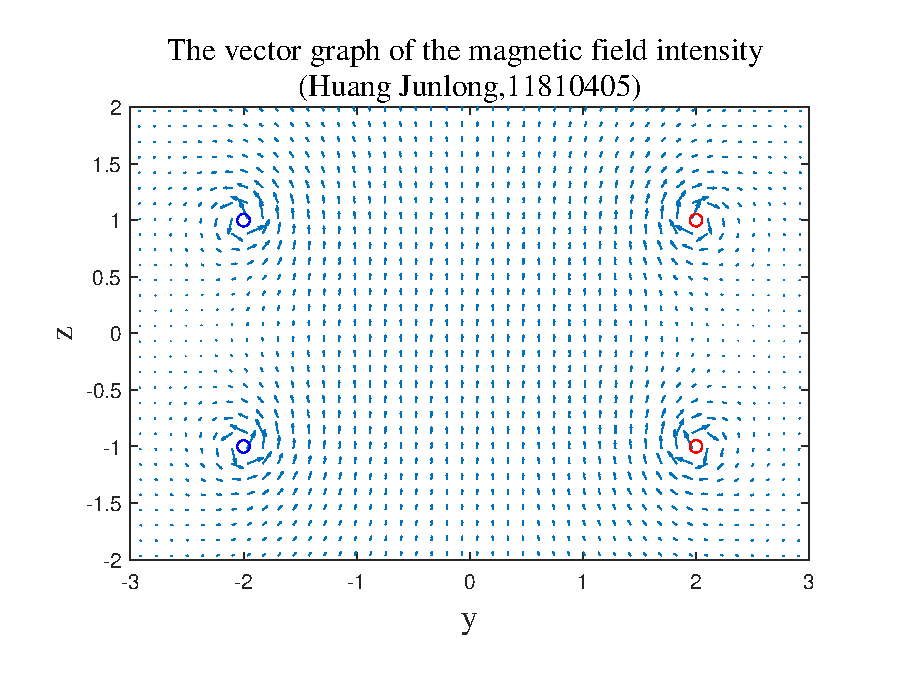
\includegraphics[width=0.9\linewidth]{F1-1.eps}
	\caption{The vector graph of the magnetic field intensity for two current loops with the same current direction}	  
	\label{fig3} 
\end{figure}
The small red circle indicates that the circuit is facing inward along the paper. From the rule of the right-hand spiral, the direction of the magnetic field around it is clockwise. On the contrary, the small blue circle indicates that the circuit direction is facing outward from the paper, and the surrounding magnetic field is counterclockwise. 

It can be seen from the figure that the magnetic field located near the center of the $ xy $ plane( for the region $ y=[-2,2], z=[-1,1] $ ) is approximately uniformly distributed.

The magnetic field intensity magnitude distributions in the space between the two current loops are as follows:
\begin{figure}[H]   
	\centering	  
	\subfloat[]{       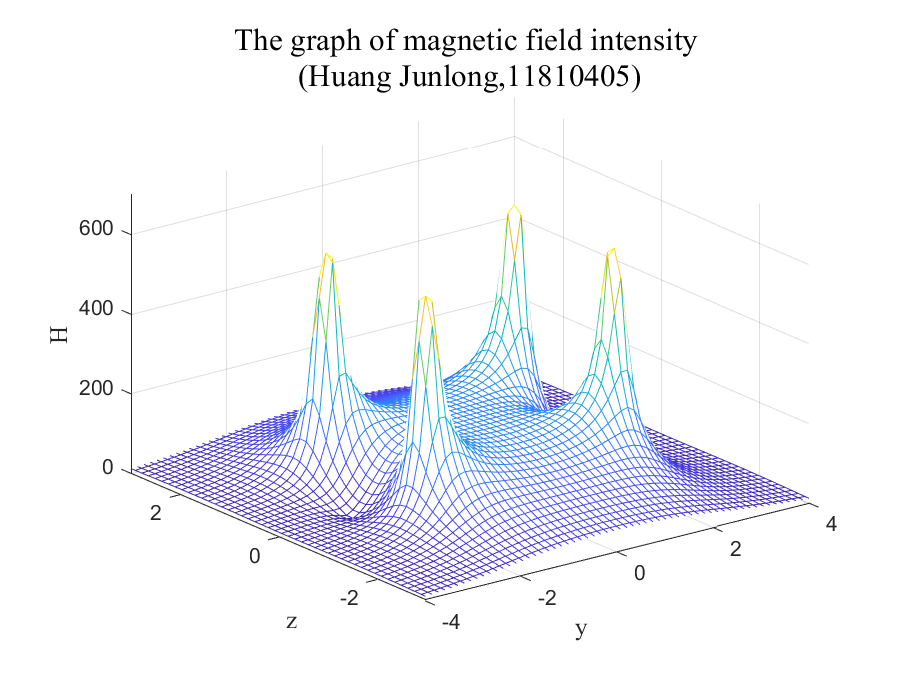
\includegraphics[width=0.45\linewidth]{F1-2.eps}}    \label{1a}\hfill	  
	\subfloat[]{        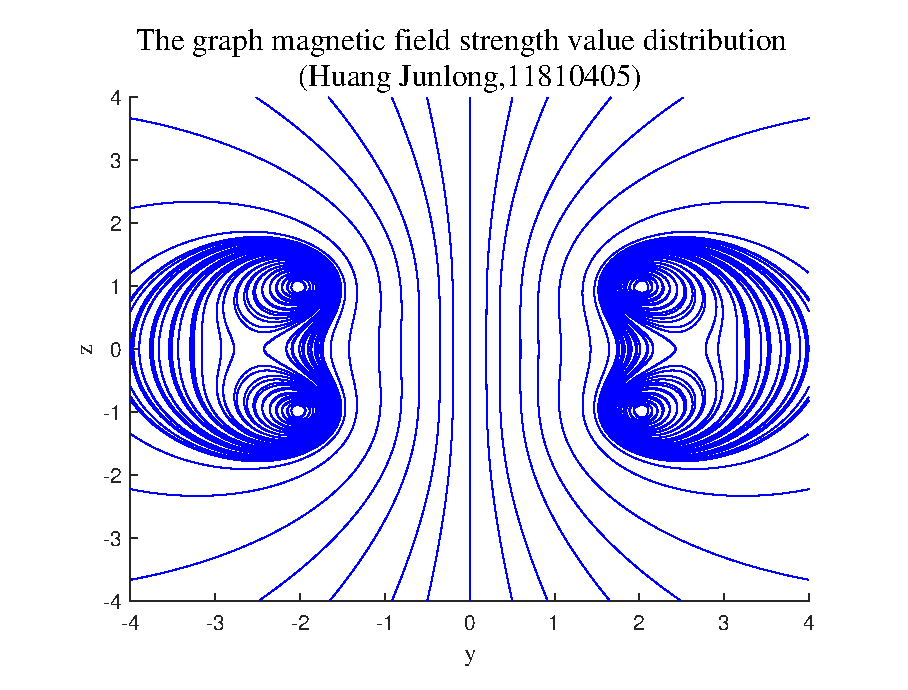
\includegraphics[width=0.45\linewidth]{F1-3.eps}}    
	\label{1b}
	\caption{Two current loops with the same current direction: (a) The graph of magnetic field intensity, (b) The graph magnetic field  intensity value distribution}	  
	\label{fig4} 
\end{figure}
The Fig. 4 shows that the magnetic field intensity magnitude distribution in the space between the two current loops is flat, and the field strength value distribution lines are approach to straight line.

For two parallelly placed current loops, when the distance between them is equal to their radius, this two-current-loops system is usually called Helmholtz coils.\cite{num2}  One characteristic of the Helmholtz coils is that the spatial magnetic field distribution between these two current loops is very uniform. To verify this conclusion,  draw the electric field intensity of the area between the current loops separately along the y direction and along the z direction.
\begin{figure}[H]   
	\centering	        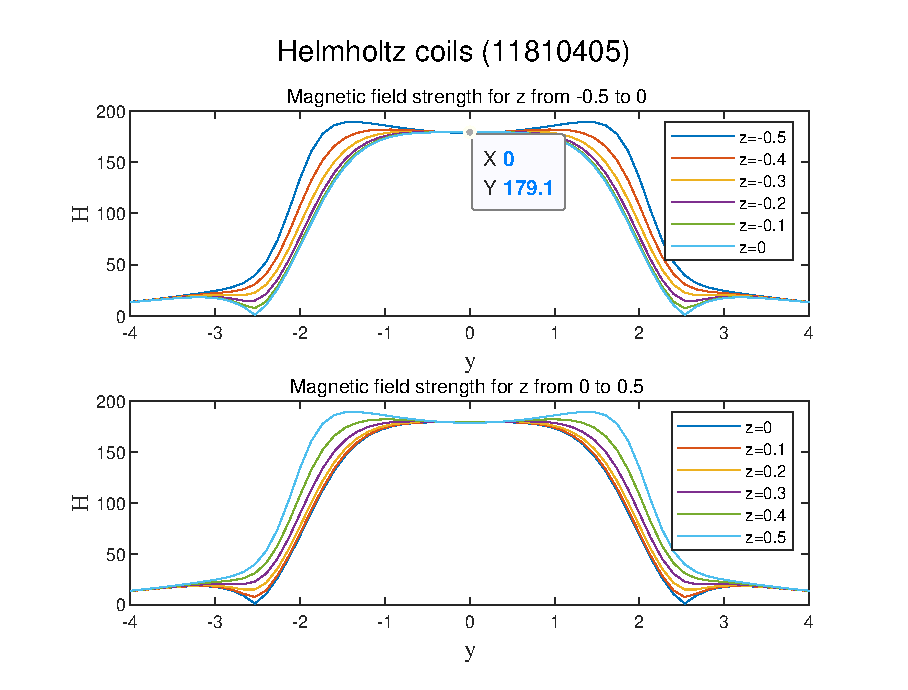
\includegraphics[width=0.9\linewidth]{F3-1.eps}
	\caption{The vector graph of the magnetic field intensity for two current loops  between these two current loops with the same current direction }	  
	\label{fig5} 
\end{figure}
Between the current loops ($ y=[-2,2] $ region), the magnetic field intensity distribution line along the y direction is almost horizontally distributed, indicating that the magnetic field along the y direction is approximately a uniform magnetic field, and the closer to the center, the more uniform the magnetic field. At the same time, along the z direction, it can also be seen that the closer to the center, the more uniform the magnetic field. 

In the central area ($ z =[-0.5,0.5] $ region), multiple magnetic field intensity distribution lines coincide, indicating that z takes different values and the magnetic field intensity is almost the same. The magnetic field distribution in the z direction is also uniform.

It can also be seen from the figure that the uniform magnetic field intensity is very close to the magnetic field intensity at the origin. The field intensity at the origin can be easily calculated by formula 2:
\begin{align}
\mathbf{H}=2\cdot \dfrac{Ia^2\mathbf{a}_z}{2(a^2+z_0^2)^{3/2}}=\dfrac{500\times2^2}{(2^2+1^2)^{3/2}}\mathbf{a}_z=\dfrac{400}{\sqrt{5}}\mathbf{a}_z=178.89\mathbf{a}_z\notag
\end{align}
It can be seen that the theoretical results are very close to the simulation results.

As can be seen from the above simulation, the middle magnetic field distribution of the Helmholtz coils is very uniform.

\subsection{Two current loops with the opposite current direction}
When the upper and lower current loops are in the opposite direction, they do not form the Helmholtz coils. Assume the upper coil current direction is counterclockwise and the lower coil current direction is clockwise. The magnetic field intensity vector distribution are as shown in Fig. 6
\begin{figure}[H]   
	\centering	        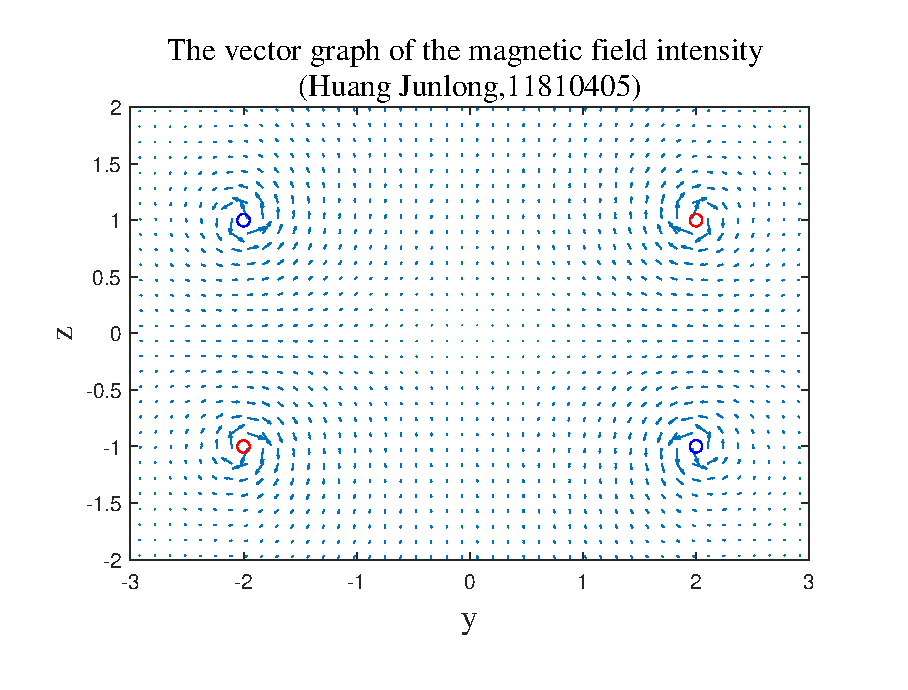
\includegraphics[width=0.9\linewidth]{F2-1.eps}
	\caption{The vector graph of the magnetic field intensity for two current loops with the opposite current direction}	  
	\label{fig6} 
\end{figure}
The small red circle indicates that the circuit is facing inward along the paper. From the rule of the right-hand spiral, the direction of the magnetic field around it is clockwise. On the contrary, the small blue circle indicates that the circuit direction is facing outward from the paper, and the surrounding magnetic field is counterclockwise. 

The magnetic field intensity magnitude distributions in the space between the two current loops are as follows:
\begin{figure}[H]   
	\centering	  
	\subfloat[]{       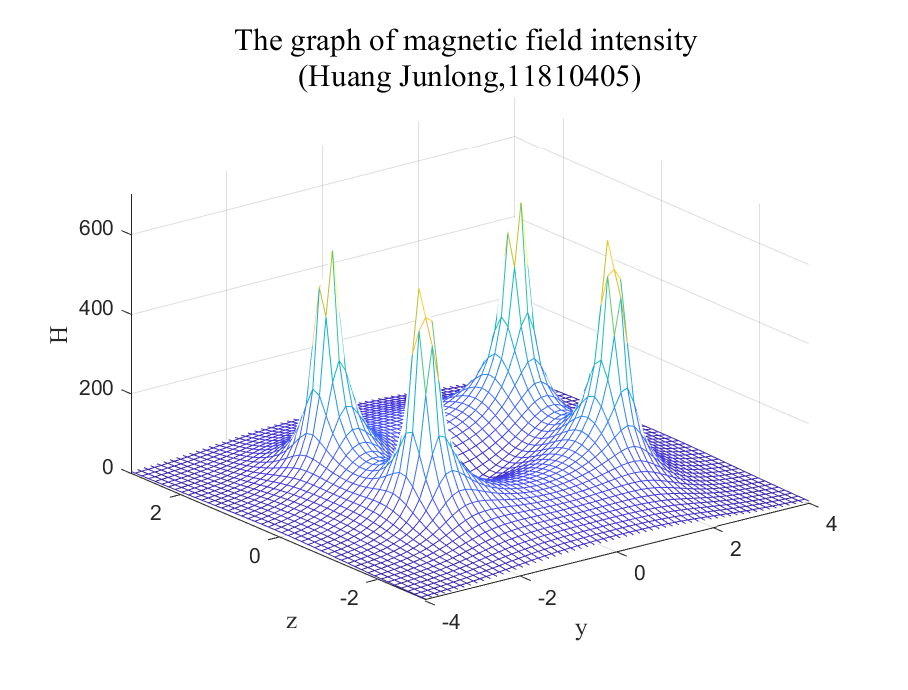
\includegraphics[width=0.45\linewidth]{F2-2.eps}}    \label{1a}\hfill	  
	\subfloat[]{        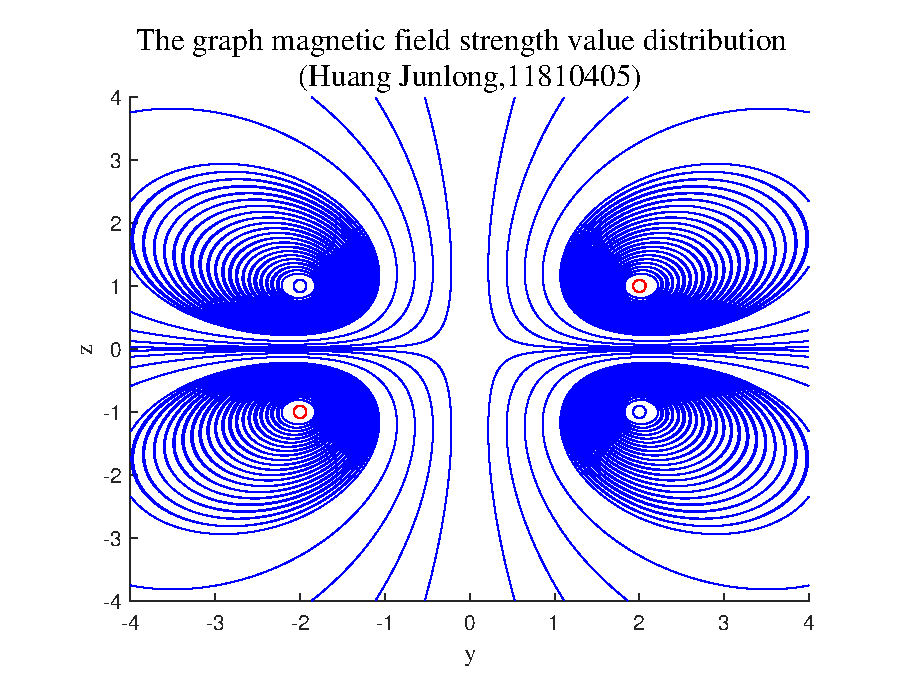
\includegraphics[width=0.45\linewidth]{F2-3.eps}}    
	\label{1b}
	\caption{Two current loops with the opposite current direction: (a) The graph of magnetic field intensity, (b) The graph magnetic field  intensity value distribution}	  
	\label{fig7} 
\end{figure}
It can be seen that the regional magnetic field intensity distribution between the current loops is no longer uniform.

In order to see this feature more clearly, several magnetic field  intensity lines specific to the central region are also drawn as follows:
\begin{figure}[H]   
	\centering	        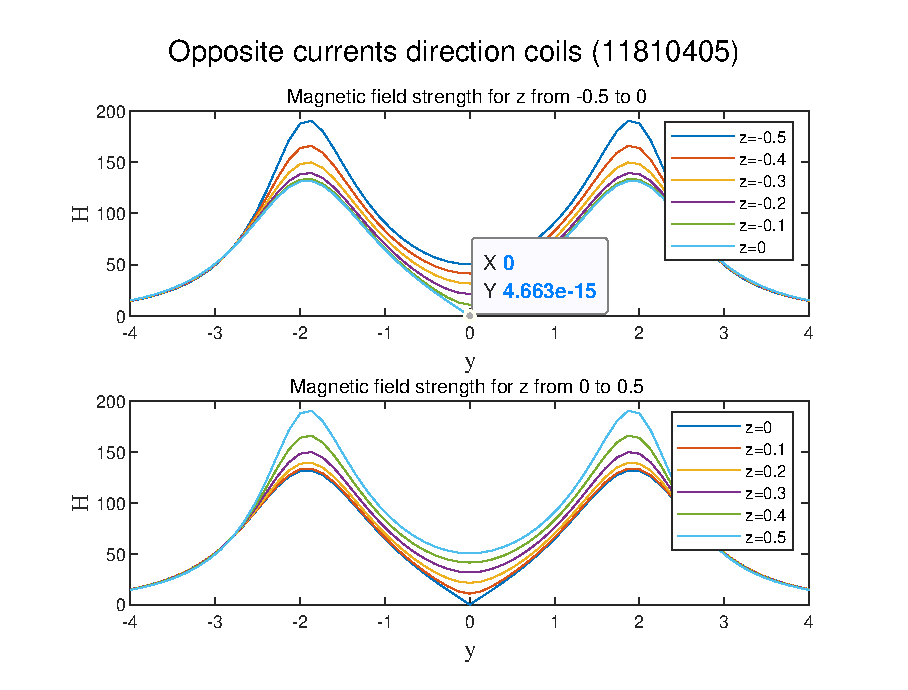
\includegraphics[width=0.9\linewidth]{F3-2.eps}
	\caption{The vector graph of the magnetic field intensity for two current loops  between these two current loops with the opposite current direction }	  
	\label{fig8} 
\end{figure}
It can be seen from theoretical analysis that the magnetic field intensityat the origin is zero. The simulation results are consistent with the theory. Compared with Fig. 5, 
It can be found that there is a significant difference between the magnetic field distribution with Helmholtz coils.
%\begin{figure}[H]   
%	\centering	  
%	\subfloat[Actuality]{       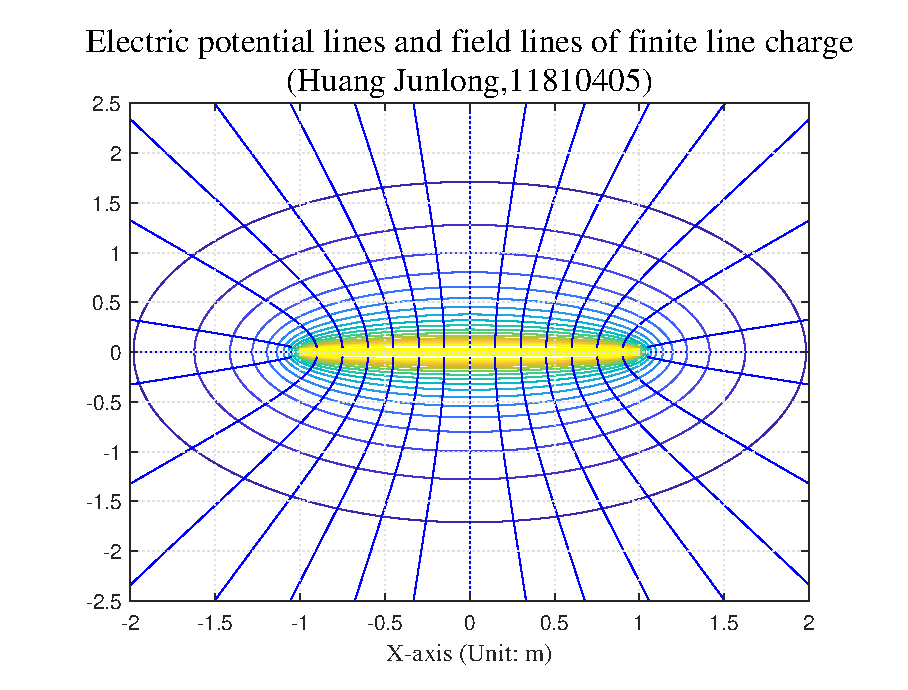
\includegraphics[width=0.45\linewidth]{Fig1-2.eps}}    \label{12}\hfill	  
%	\subfloat[n=20]{        \includegraphics[width=0.45\linewidth]{Fig2-2.eps}}    
%	\label{22}\\
%	\subfloat[n=50]{       \includegraphics[width=0.45\linewidth]{Fig3-2.eps}}    \label{32}\hfill	  
%	\subfloat[n=100]{        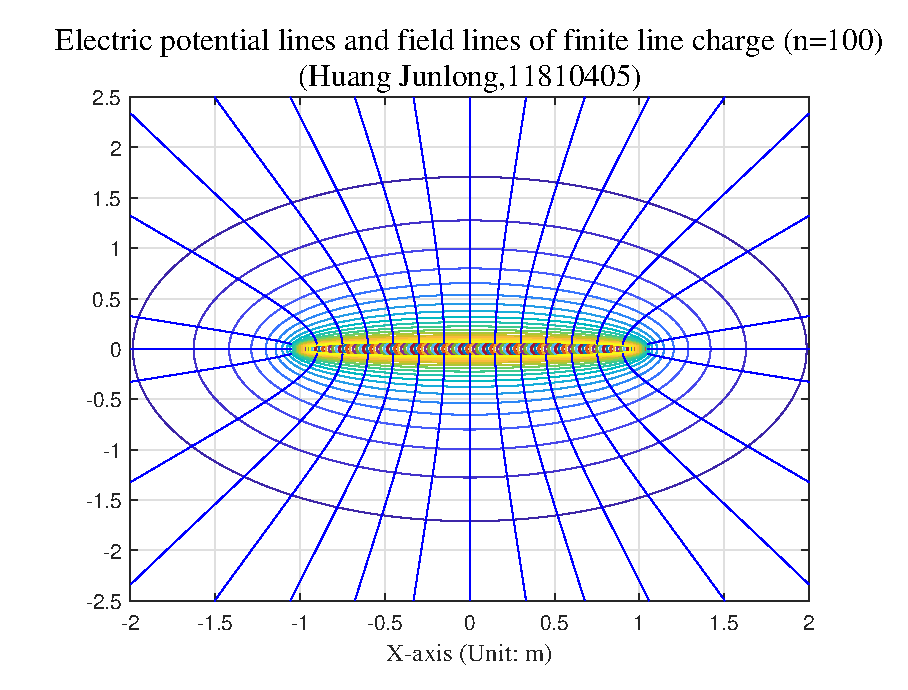
\includegraphics[width=0.45\linewidth]{Fig4-2.eps}}    
%	\label{42}\\
%	\caption{The potential and the electric field distribution of the finite line chargeas (a) The actually result calculated by Calculus Method (b) The approximate result calculated by Infinitesimal Method when n=20 (c) n=50 (d) n=100
%	}	  
%	\label{fig4} 
%\end{figure}
\newpage
\section{Conclusion}
Through theoretical calculation and Matlab simulation, two identical current loops parallel to the $ xy $ plane are derived from the distribution of magnetic fields in space in the same direction of current and in the opposite case.

At the same time, the characteristics of uniform distribution of the spatial magnetic field added by the current loops are visually verified when the current direction is the same (i.e. the composition Helmholtz coils.).

The method of calculating the magnetic field intensity  distribution using Biot-Savart law and infinitesimal method can also be extended to the magnetic field distribution of other current shapes.




\bibliographystyle{IEEEtran}
\bibliography{IEEEabrv,mylib}
%\begin{thebibliography}{2}

%\bibitem{IEEEhowto:kopka}
%H.~Kopka and P.~W. Daly, \emph{A Guide to \LaTeX}, 3rd~ed.\hskip 1em plus
%  0.5em minus 0.4em\relax Harlow, England: Addison-Wesley, 1999.

%\end{thebibliography}

% biography section
% 
% If you have an EPS/PDF photo (graphicx package needed) extra braces are
% needed around the contents of the optional argument to biography to prevent
% the LaTeX parser from getting confused when it sees the complicated
% \includegraphics command within an optional argument. (You could create
% your own custom macro containing the \includegraphics command to make things
% simpler here.)
%\begin{IEEEbiography}[{\includegraphics[width=1in,height=1.25in,clip,keepaspectratio]{mshell}}]{Michael Shell}
% or if you just want to reserve a space for a photo:



% You can push biographies down or up by placing
% a \vfill before or after them. The appropriate
% use of \vfill depends on what kind of text is
% on the last page and whether or not the columns
% are being equalized.

%\vfill

% Can be used to pull up biographies so that the bottom of the last one
% is flush with the other column.
%\enlargethispage{-5in}

% that's all folks
\newpage
\onecolumn 
\begin{appendices}
\section{}
\end{appendices}

\begin{lstlisting}
%% This is the code for Lab 3
%% Parameter setting
clc,clear all                   
a=2;              % The radius of the current loop
I=500;            % The current value in the current loop
C=I/(4*pi);       % Merge the constants
N=60;             % Set the number of division
ym=4;             % Set the range of y direction in the field domain
zm=3;             % Set the range of z direction in the field domain
% zm=4 For two cases. zm=3 for magnetic analysis
y=linspace(-ym,ym,61);           % Equally divide y axis into 61 parts
z=linspace(-zm,zm,61);           % Equally divide z axis into 61 parts
theta0=linspace(0,2*pi,N+1);     % Division of the angle of circumference  

%% Two current loops
% The start point coordinate of each segment of the loop 
theta1=theta0(1:N);                               
x1=a*cos(theta1); y1=a*sin(theta1);                     
% The ending point coordinate of each segment of theloop
theta2=theta0(2:N+1);                           
x2=a*cos(theta2); y2=a*sin(theta2);    
%Calculate the 3 coordinate components of the midpoint of each segment of the loop.
zcu=a/2; zcd=-a/2; xc=(x2+x1)./2; yc=(y2+y1)./2;   
% Calculate the 3 length components of each segment vector dl.
dlz=0;dlx=x2-x1;dly=y2-y1;
NGx=61; NGy=61;                           % Grid dimension
Hy=zeros(20);Hz=zeros(20);H=zeros(20);    % Construct the H matrix
Hyoppo=zeros(20);Hzoppo=zeros(20);Hoppo=zeros(20); % Construct the H matrix

for i=1:NGy       % Loop computation of the value of H(x,y) in each grid
for j=1:NGx
% Calculate the 3 length components of the radius vector r,
rx=0-xc; ry=y(j)-yc; rzu=z(i)-zcu; rzd=z(i)-zcd;                  
% Calculate r cube
r3u=sqrt(rx.^2+ry.^2+rzu.^2).^3;
r3d=sqrt(rx.^2+ry.^2+rzd.^2).^3;
% Calculate the y, z components of the cross product dlxr,
dlXr_yu=dlz.*rx-dlx.*rzu; dlXr_yd=dlz.*rx-dlx.*rzd;
dlXr_zu=dlx.*ry-dly.*rx; dlXr_zd=dlx.*ry-dly.*rx;
% Accumulate the magnetic field intensity created by each segment of the loop.
% For the same direction, use `+`; For the opposite direction, use `-`
Hy(i,j)=sum(C.*dlXr_yu./r3u)+sum(C.*dlXr_yd./r3d);                
Hz(i,j)=sum(C.*dlXr_zu./r3u)+sum(C.*dlXr_zd./r3d);
%%%
Hyoppo(i,j)=sum(C.*dlXr_yu./r3u)-sum(C.*dlXr_yd./r3d);                
Hzoppo(i,j)=sum(C.*dlXr_zu./r3u)-sum(C.*dlXr_zd./r3d);
%%%
H=(Hy.^2+Hz.^2).^0.5;           %Calculate the magnitude of H
Hoppo=(Hyoppo.^2+Hzoppo.^2).^0.5;         
end
end

%% For two current loops with the same current direction
% Plot the vector graph of the magnetic field intensity
figure
quiver(y,z,Hy,Hz);                    
hold on     
axis equal
axis([-3,3,-2,2]); 
plot(2,1,'ro',-2,1,'bo'),        % Standard coil section
plot(2,-1,'ro',-2,-1,'bo'),        % Standard coil section
xlabel('y','FontName','Times New Roman','fontsize',16),
ylabel('z','FontName','Times New Roman','fontsize',16),   
title({['The vector graph of the magnetic field intensity '],...
['(Huang Junlong,11810405)']} ,'FontName','Times New Roman', 'fontsize', 15);

% Plot the graph of magnetic field intensity
figure
mesh(y,z,H);   
axis([-4,4,-3,3,0,700])   
xlabel('y','FontName','Times New Roman','fontsize',12),
ylabel('z','FontName','Times New Roman','fontsize',12),
zlabel('H','FontName','Times New Roman','fontsize',12);
title({['The graph of magnetic field intensity '],...
['(Huang Junlong,11810405)']} ,'FontName','Times New Roman', 'fontsize', 15);

% The graph magnetic field strength value distribution 
figure
theta=[0 20 50 60 80 90 100 120 130 160 180].*pi/180;  %Set the radian value of the streamlines
ysu=2.1*cos(theta);     % Set the streamline starting circle?s y coordinate
zsu=2.1*sin(theta)+1;   % Set the streamline starting circle?s z coordinate
streamline(y,z,Hy,Hz,ysu,zsu);  % Outwardly plot the magnetic line of force 	
streamline(y,z,-Hy,-Hz,ysu,zsu);   % Inwardly plot the magnetic line of force 
ysd=2.1*cos(theta);     % Set the streamline starting circle?s y coordinate
zsd=2.1*sin(theta)-1;   % Set the streamline starting circle?s z coordinate
streamline(y,z,Hy,Hz,ysd,zsd);  % Outwardly plot the magnetic line of force 	
streamline(y,z,-Hy,-Hz,ysd,zsd);   % Inwardly plot the magnetic line of force 
xlabel('y','FontName','Times New Roman','fontsize',12),
ylabel('z','FontName','Times New Roman','fontsize',12);
title({['The graph magnetic field strength value distribution  '],...
['(Huang Junlong,11810405)']} ,'FontName','Times New Roman', 'fontsize', 15);

%% For two current loops with the opposite current direction
% Plot the vector graph of the magnetic field intensity
figure
quiver(y,z,Hyoppo,Hzoppo);                    
hold on     
axis equal
axis([-3,3,-2,2]); 
plot(2,1,'ro',-2,1,'bo'),        % Standard coil section
plot(2,-1,'bo',-2,-1,'ro'),        % Standard coil section
xlabel('y','FontName','Times New Roman','fontsize',16),
ylabel('z','FontName','Times New Roman','fontsize',16),   
title({['The vector graph of the magnetic field intensity '],...
['(Huang Junlong,11810405)']} ,'FontName','Times New Roman', 'fontsize', 15);

% Plot the graph of magnetic field intensity
figure
mesh(y,z,Hoppo);   
axis([-4,4,-3,3,0,700])   
xlabel('y','FontName','Times New Roman','fontsize',12),
ylabel('z','FontName','Times New Roman','fontsize',12),
zlabel('H','FontName','Times New Roman','fontsize',12);
title({['The graph of magnetic field intensity '],...
['(Huang Junlong,11810405)']} ,'FontName','Times New Roman', 'fontsize', 15);

% The graph magnetic field strength value distribution 
figure
theta=[5 50 60 70 80 90 100 110 120 130 175].*pi/180;  %Set the radian value of the streamlines
ysu=2.1*cos(theta);     % Set the streamline starting circle?s y coordinate
zsu=2.1*sin(theta)+1;   % Set the streamline starting circle?s z coordinate
streamline(y,z,Hyoppo,Hzoppo,ysu,zsu);  % Outwardly plot the magnetic line of force 	
streamline(y,z,-Hyoppo,-Hzoppo,ysu,zsu);   % Inwardly plot the magnetic line of force 
ysd=2.1*cos(theta+pi);     % Set the streamline starting circle?s y coordinate
zsd=2.1*sin(theta+pi)-1;   % Set the streamline starting circle?s z coordinate
streamline(y,z,Hyoppo,Hzoppo,ysd,zsd);  % Outwardly plot the magnetic line of force 	
streamline(y,z,-Hyoppo,-Hzoppo,ysd,zsd);   % Inwardly plot the magnetic line of force 
hold on
plot(2,1,'ro',-2,1,'bo'),        % Standard coil section
plot(2,-1,'bo',-2,-1,'ro'),        % Standard coil section
xlabel('y','FontName','Times New Roman','fontsize',12),
ylabel('z','FontName','Times New Roman','fontsize',12);
title({['The graph magnetic field strength value distribution  '],...
['(Huang Junlong,11810405)']} ,'FontName','Times New Roman', 'fontsize', 15);

%% Magnetic field strength in the space between the two current loops
% For Helmholtz coil
figure
for i=26:31
subplot(2,1,1) % The calculate result for z coordinate.
plot(y,H(i,:)) % The magnetic along the y axis
hold on
end
xlabel('y','FontName','Times New Roman','fontsize',12),
ylabel('H','FontName','Times New Roman','fontsize',12);
title('Magnetic field strength for z from -0.5 to 0 ')
legend('z=-0.5','z=-0.4','z=-0.3','z=-0.2','z=-0.1','z=0')
for k=31:36 
subplot(2,1,2)
plot(y,H(k,:))
hold on
end
xlabel('y','FontName','Times New Roman','fontsize',12),
ylabel('H','FontName','Times New Roman','fontsize',12);
title('Magnetic field strength for z from 0 to 0.5 ')
legend('z=0','z=0.1','z=0.2','z=0.3','z=0.4','z=0.5')
suptitle('Helmholtz coils (11810405)')

% For opposite direction currents 
figure
subplot(2,1,1)
for i=26:31
plot(y,Hoppo(i,:))
hold on
end
xlabel('y','FontName','Times New Roman','fontsize',12),
ylabel('H','FontName','Times New Roman','fontsize',12);
title('Magnetic field strength for z from -0.5 to 0 ')
legend('z=-0.5','z=-0.4','z=-0.3','z=-0.2','z=-0.1','z=0')
subplot(2,1,2)
for k=31:36
plot(y,Hoppo(k,:))
hold on
end
xlabel('y','FontName','Times New Roman','fontsize',12),
ylabel('H','FontName','Times New Roman','fontsize',12);
title('Magnetic field strength for z from 0 to 0.5 ')
legend('z=0','z=0.1','z=0.2','z=0.3','z=0.4','z=0.5')
suptitle('Opposite currents direction coils (11810405)')
%% end
\end{lstlisting}


\end{document}

